\documentclass{article}   	                         % use "amsart" instead of "article" for AMSLaTeX format
\usepackage{fullpage}                		% ... or a4paper or a5paper or ... 
\usepackage{enumerate}				% Use enumerate to list subsections
\usepackage{graphicx}				% Use pdf, png, jpg, or eps§ with pdflatex; use eps in DVI mode
\usepackage{fancyvrb}
\usepackage{amsmath}
\usepackage{dsfont}
\usepackage{pgfgantt}
\usepackage{pgfplots}
\newcommand{\ra}{\rightarrow}

%SetFonts

\title{Computer System Fundamentals HW \#1}
\author{Quan Zhou}
\date{Feb 1st, 2016}
\begin{document}
\maketitle
\section*{Problem 1}
\begin{enumerate}[(a)]
\item 
\tikzset{every picture/.style={xscale=0.57, yscale= 0.57, transform shape}}
\begin{ganttchart}[
vgrid,
hgrid,
inline,
milestone inline label node/.append style={left=5mm}
]{1}{40}
\gantttitle{A Batch Processing System (BPS) with MPL = 1}{40} \\
\ganttgroup{Period of Time}{1}{19} \\
  \ganttbar[bar/.append style={fill=red!50}]{I}{1}{2}
  \ganttbar[bar/.append style={fill=green!50}]{I}{20}{21} 
  \ganttbar[bar/.append style={fill=red!50}]{III}{11}{12}
  \ganttbar[bar/.append style={fill=green!50}]{III}{30}{31}
  \ganttbar[bar/.append style={fill=red!50}]{V}{19}{19}
  \ganttbar[bar/.append style={fill=green!50}]{V}{38}{38} \\
  \ganttbar[bar/.append style={fill=red!50}]{II}{3}{10}
  \ganttbar[bar/.append style={fill=green!50}]{II}{22}{29}  \\
  \ganttbar[bar/.append style={fill=red!50}]{IV}{13}{18}
  \ganttbar[bar/.append style={fill=green!50}]{IV}{32}{37}  \\
  \ganttmilestone{Request 1 Completed}{19} \\
  \ganttmilestone{Request 2 Completed}{38} \\
\end{ganttchart}
\\
\\
From the above chart, we see that the usage for CPU, disk, and network are 5 msec, 8 msec and 6 msec respectively. The total span of time to process this one request is 19 msec. Therefore, utilization of each resources are $\frac{5}{19}$,  $\frac{8}{19}$, $\frac{6}{19}$, or $26.3\%$, $42.1\%$, $31.6\%$. 
\item
$ Bandwidth =  \frac{1}{19}$ or 52.6 \text {  requests/sec}

\item
\begin{ganttchart}[
vgrid,
hgrid,
inline,
milestone inline label node/.append style={left=5mm}
]{1}{62}
\gantttitle{A Batch Processing System (BPS) with MPL $\geq$ 2}{62} \\
\ganttgroup{Period of Time for one request}{22}{47} \\
  \ganttbar[bar/.append style={fill=red!50}]{I}{1}{2}
  \ganttbar[bar/.append style={fill=green!50}]{I}{3}{4}
  \ganttbar[bar/.append style={fill=yellow!50}]{I}{22}{23}
  \ganttbar[bar/.append style={fill=blue!50}]{I}{35}{36}
  \ganttbar[bar/.append style={fill=pink!50}]{I}{48}{49}
  \ganttbar[bar/.append style={fill=brown!50}]{I}{61}{62}  
  \ganttbar[bar/.append style={fill=red!50}]{III}{11}{12}
  \ganttbar[bar/.append style={fill=green!50}]{III}{19}{20}
  \ganttbar[bar/.append style={fill=yellow!50}]{III}{32}{33}
  \ganttbar[bar/.append style={fill=blue!50}]{III}{45}{46}
  \ganttbar[bar/.append style={fill=pink!50}]{III}{58}{59}    
  \ganttbar[bar/.append style={fill=red!50}]{V}{21}{21}
  \ganttbar[bar/.append style={fill=green!50}]{V}{34}{34}
  \ganttbar[bar/.append style={fill=yellow!50}]{V}{47}{47}
  \ganttbar[bar/.append style={fill=blue!50}]{V}{60}{60} \\
  \ganttbar[bar/.append style={fill=red!50}]{II}{3}{10}
  \ganttbar[bar/.append style={fill=green!50}]{II}{11}{18}
  \ganttbar[bar/.append style={fill=yellow!50}]{II}{24}{31}
  \ganttbar[bar/.append style={fill=blue!50}]{II}{37}{44}
  \ganttbar[bar/.append style={fill=pink!50}]{II}{50}{57} \\
  \ganttbar[bar/.append style={fill=red!50}]{IV}{13}{18}
  \ganttbar[bar/.append style={fill=green!50}]{IV}{21}{26}
  \ganttbar[bar/.append style={fill=yellow!50}]{IV}{34}{39}
  \ganttbar[bar/.append style={fill=blue!50}]{IV}{47}{52}
  \ganttbar[bar/.append style={fill=pink!50}]{IV}{60}{65} \\
  \ganttmilestone{Request 1 Completed}{21} \\
  \ganttmilestone{Request 2 Completed}{34} \\
  \ganttmilestone{Request 3 Completed}{47} \\
  \ganttmilestone{Request 4 Completed}{60} \\
\end{ganttchart}
\\
For N = 2: We assume that the more progressed requests are prioritized to the less progressed requests. From the above chart, we see that the usage for CPU, disk, and network are 10 msec, 16 msec and 12 msec respectively.  The period of time to complete one process when N = 2 is 26 msec. Utilization of each resources can be found by following the definition and we get $\frac{10}{26}$,  $\frac{16}{26}$, $\frac{12}{26}$, or $38.5\%$, $61.5\%$, $46.2\%$. 
\item
$ Bandwidth =  \frac{2}{26}$ or 76.9 \text {  requests/sec}
\item
\begin{ganttchart}[
vgrid,
hgrid,
inline,
milestone inline label node/.append style={left=5mm}
]{1}{58}
\gantttitle{A Batch Processing System (BPS) with MPL $\geq$ 2; N = 3}{58} \\
\ganttgroup{Period of Time for one request}{22}{45} \\
  \ganttbar[bar/.append style={fill=red!50}]{I}{1}{2}
  \ganttbar[bar/.append style={fill=green!50}]{I}{3}{4}
  \ganttbar[bar/.append style={fill=yellow!50}]{I}{5}{6}
  \ganttbar[bar/.append style={fill=blue!50}]{I}{22}{23}
  \ganttbar[bar/.append style={fill=pink!50}]{I}{30}{31}
  \ganttbar[bar/.append style={fill=orange!50}]{I}{38}{39}
  \ganttbar[bar/.append style={fill=brown!50}]{I}{46}{47}
  \ganttbar[bar/.append style={fill=gray!50}]{I}{54}{55}      
  \ganttbar[bar/.append style={fill=red!50}]{III}{11}{12}
  \ganttbar[bar/.append style={fill=green!50}]{III}{19}{20}
  \ganttbar[bar/.append style={fill=yellow!50}]{III}{27}{28}
  \ganttbar[bar/.append style={fill=blue!50}]{III}{35}{36}
  \ganttbar[bar/.append style={fill=pink!50}]{III}{43}{44}
  \ganttbar[bar/.append style={fill=orange!50}]{III}{51}{52}    
  \ganttbar[bar/.append style={fill=red!50}]{V}{21}{21}
  \ganttbar[bar/.append style={fill=green!50}]{V}{29}{29}
  \ganttbar[bar/.append style={fill=yellow!50}]{V}{37}{37}
  \ganttbar[bar/.append style={fill=blue!50}]{V}{45}{45}
  \ganttbar[bar/.append style={fill=pink!50}]{V}{53}{53} \\
  \ganttbar[bar/.append style={fill=red!50}]{II}{3}{10}
  \ganttbar[bar/.append style={fill=green!50}]{II}{11}{18}
  \ganttbar[bar/.append style={fill=yellow!50}]{II}{19}{26}
  \ganttbar[bar/.append style={fill=blue!50}]{II}{27}{34}
  \ganttbar[bar/.append style={fill=pink!50}]{II}{35}{42}
  \ganttbar[bar/.append style={fill=orange!50}]{II}{43}{50}
  \ganttbar[bar/.append style={fill=brown!50}]{II}{51}{58} \\
  \ganttbar[bar/.append style={fill=red!50}]{IV}{13}{18}
  \ganttbar[bar/.append style={fill=green!50}]{IV}{21}{26}
  \ganttbar[bar/.append style={fill=yellow!50}]{IV}{29}{34}
  \ganttbar[bar/.append style={fill=blue!50}]{IV}{37}{42}
  \ganttbar[bar/.append style={fill=pink!50}]{IV}{45}{50}
  \ganttbar[bar/.append style={fill=orange!50}]{IV}{53}{58} \\
  \ganttmilestone{Request 1 Completed}{21} \\
  \ganttmilestone{Request 2 Completed}{29} \\
  \ganttmilestone{Request 3 Completed}{37} \\
  \ganttmilestone{Request 4 Completed}{45} \\
  \ganttmilestone{Request 5 Completed}{53} \\
\end{ganttchart}
\\
From the above chart, we see that the usage for CPU, disk, and network are 15 msec, 24 msec and 18 msec respectively in a total span of 24 msec. Utilization of each resources can be found by following the definition and we get $\frac{15}{24}$,  $\frac{24}{24}$, $\frac{18}{24}$, or $62.5\%$, $100\%$, $75\%$. 
\\
\\
$ Bandwidth =  \frac{3}{24}$ or 125 requests/sec
\item
We know that the disk has hit $100 \%$ utilization, then the maxx capacity is equal to the bandwidth found in part (e) which is :
125 requests/sec
\\
\item
The bottleneck resource is the disk: as N increases, the utilization of the disk would first approach to $100\%$. This limits the throughput of this system.
\\
\end{enumerate}

\section*{Problem 2}
\begin{enumerate}[(a)]
\item
$F_{CPU} = \frac{5 msec}{19 msec} = \frac{5}{19} $, and $ S = r $ \\
Using Amdahl's Law, we have:\\
System Overall Speedup  = $ \frac{1}{1 - \frac{5}{19} + \frac{5}{19*r}} $ = $\frac{1}{\frac{14}{19} + \frac{5}{19*r}} $\\
\\
\begin{tikzpicture}
\begin{axis}[
    axis lines = left,
    xlabel = $r$,
    ylabel = {Overall Speedup},
    legend pos = outer north east,
]
%Below is the Overall Speedup as a function of CPU speed increase
\addplot [
    domain=1:20, 
    samples= 100, 
    color=black,   
]
{1/(14/19+5/(19*x))};
\addlegendentry{Overall Speedup as a function of CPU speed increase}
\end{axis}
\end{tikzpicture}
\\
\item
Assume CPU can infinitely fast, then the value of r increases to $\infty$. From the function from part (a), we are left with Overall Speedup = $\frac{1}{\frac{14}{19}}$  = $\frac{19}{14}$ or 1.36. And that is our theoretical limit.
\\ 
\item
$F_{disk} = \frac{8 msec}{19 msec} = \frac{8}{19} $, and $ S = r $ \\
Using Amdahl's Law, we have:\\
System Overall Speedup (disk)  = $ \frac{1}{1 - \frac{8}{19} + \frac{8}{19*r}} $ = $\frac{1}{\frac{11}{19} + \frac{8}{19*r}} $\\
Assume the disk can infinitely fast, then the value of r increases to $\infty$. From the equation above, we can find the theoretical limit for the speedup is = $\frac{1}{\frac{11}{19}}$  = $\frac{19}{11}$ or 1.73. And that is our theoretical limit.
\\
$F_{network} = \frac{6 msec}{19 msec} = \frac{5}{19} $, and $ S = r $ \\
Using Amdahl's Law, we have:\\
System Overall Speedup (network)  = $ \frac{1}{1 - \frac{6}{19} + \frac{6}{19*r}} $ = $\frac{1}{\frac{13}{19} + \frac{6}{19*r}} $\\
Assume the network can infinitely fast, then the value of r increases to $\infty$. From the equation above, we can find the theoretical limit for the speedup is = $\frac{1}{\frac{13}{19}}$  = $\frac{19}{13}$ or 1.46. And that is our theoretical limit.\\
\\
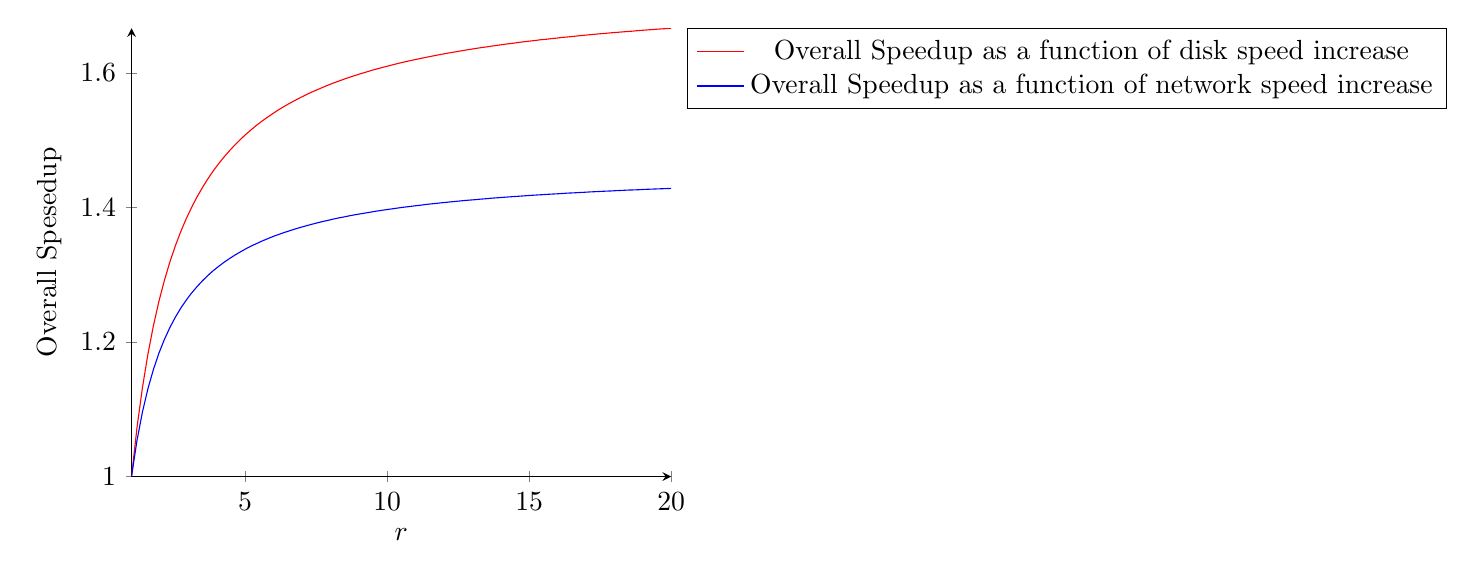
\begin{tikzpicture}
\begin{axis}[
    axis lines = left,
    xlabel = $r$,
    ylabel = {Overall Spesedup},
    legend pos = outer north east,
]
%Below is the Overall Speedup as a function of disk speed increase
\\
\\
\addplot [
    domain=1:20, 
    samples= 100, 
    color=red,
]
{1/(11/19+8/(19*x))};
\addlegendentry{Overall Speedup as a function of disk speed increase}

%Below is the Overall Speedup as a function of network speed increase is defined
\addplot [
    domain=1:20, 
    samples= 100, 
    color=blue,
]
{1/(13/19+6/(19*x))};
\addlegendentry{Overall Speedup as a function of network speed increase}
\end{axis}
\end{tikzpicture}
\\
\item
The minimum speedup for the various device to achieve equal utilization of all resources is to increase the speed of the disk, which has the higher utilization among the three resources of this web server system. Current utilization of the disk is 8 msec for every request; if we speed up the disk to 5 msec for every request, and likewise speed up the network also to 5 msec so the utilization for all three resources are equal, then we could get an overall speedup of 1.19 and 1.05 respectively.
\item
Since all three resources/devices have equal utilization, the resulting capacity is the max throughput of any device and therefore equals to $\frac{1}{5}$ or 200 requests/sec
\end{enumerate}

\section*{Problem 3}
\begin{enumerate}[(a)]
\item
\begin{BVerbatim}
I. cut the latency of the main memory by 1/2
II. cut the latency of the cache by 1/5
\end{BVerbatim}
\\
\\
The expected execution time without improvement is:
\begin{align*}
 \mathds{E}(T)
 & = \mathds{P}(X = cache hit)\cdot (T_{hit}) +  \mathds{P}(X = cache miss)\cdot (T_{miss}) 
 \\& = (95\%)\cdot(1) + (5\%)\cdot(8)
 \\& = 1.35 \text {  units of time}
\end{align*}
Now, with improvement I, the execution time is:
\begin{align*}
 \mathds{E}(T_{I})
& = (95\%)\cdot(1) + (5\%)\cdot(4)
 \\& = 0.95 + 0.20
 \\& = 1.15 \text {  units of time}
\end{align*}
therefore achieving a speedup of $\frac{1.35}{1.15} = 1.17$
\\
versus, with improvement II:
\begin{align*}
 \mathds{E}(T_{II})
& = (95\%)\cdot(0.8) + (5\%)\cdot(8)
 \\& = 0.76 + 0.40
 \\& = 1.16 \text {  units of time}
\end{align*}
therefore achieving a speedup of $\frac{1.35}{1.16} = 1.16$\\
\item
Since the choice to optimized the cache or main memory may change as the cache hit rate varies, we have the follow equation:\\
Given hit rate = h, and therefore miss rate = 1 - h, we have:
$h\cdot(1) +  (1 - h)\cdot (4)$ = $h\cdot(0.8) + (1 - h)\cdot (8)$
$4.2\cdot h = 4$
so h = $\frac{20}{21}$
this number means that if the cache hit rate is less than $\frac{20}{21}$, cutting the latency of the main memory (improvement I) would be a better choice whereas if the cache hit rate is more than $\frac{20}{21}$, improving the cache latency (improvement II) would be a better choice.\\
\item
\begin{align*}
 Speedup
 & = \frac{\mathds{E}(T)}{\mathds{E}(T_{I + II})}
 \\& = \frac{h\cdot (1) + (1 - h)\cdot (8)}{h\cdot (0.8) + (1 - h)\cdot (4)}
 \\& = \frac{8 -7h}{4 - 3.2h}
\end{align*}
\end{enumerate}

\section*{Problem 4}
\begin{enumerate}[(a)]
\item
Since the percentage of payload for each packet is $\frac{150}{1500}$ or $10\%$, the we have:\\
Throughput = Capacity $\times (1 - 10\%) \times (1 - P)^H$ = (10 Mbps) $\cdot (90\%) \cdot (1 - P)^H$ = $9 (1 - P)^H$ Mbps
\\
\item
For H = 1 and P = 0.01, we substitue H and P into the equation above and we obtain:\\
$9 (1 - P)^H = 9*0.99^1 = 8.91$ Mbps\\
\item
To achieve a bandwidth of more than 6 Mbps:\\
$9 (1 - P)^H > 6 $\\
$(1 - P)^H > \frac{2}{3}$\\
$1 - P > (\frac{2}{3})^{\frac{1}{H}}$
so $P < 1 - (\frac{2}{3})^{\frac{1}{H}}$
\end{enumerate}

\section*{Problem 5}
\begin{enumerate}[(a)]
\item
There are four distinctive paths between the source "A" and the destination "B" (see Figure 1). 
\begin{center}
\includegraphics[scale = 0.45]{slide1.jpg}
\end{center}
By following the algorithm given in the problem we first examine the path colored in blue (see Figure 2) 
\begin{center}
\includegraphics[scale = 0.45]{slide2.jpg}
\end{center}
The bottleneck flow in the blue path is 10 and therefore the flow capacity is 10. Since there are still augmenting paths to be added to the residual graph, we go to the next path.
\begin{center}
\includegraphics[scale = 0.45]{slide3.jpg}
\end{center}
Since the minimum flow in the purple path is 50, so the flow capacity now becomes 60 (after adding 50 from the purple path). Since there are still augmenting paths to be added to the residual graph, we go to the next path.
\begin{center}
\includegraphics[scale = 0.45]{slide4.jpg}
\end{center}
We can add another 40 to the flow capacity from the red path. 
\begin{center}
\includegraphics[scale = 0.45]{slide5.jpg}
\end{center}
Lastly, the yellow path could contribute another 50, tallying up to 150 as the max-flow in this particular network.
By following the algorithm, there are two other possible residual graphs and they are shown below. In Figure 6, the blue path was not utilized at all because there is no other augmenting path available. 
\begin{center}
\includegraphics[scale = 0.45]{slide6.jpg}
\end{center}
\begin{center}
\includegraphics[scale = 0.45]{slide7.jpg}
\end{center}
All of the residual graphs indicate that the maximum capacity is 150 for this network. 

\item
Given a residual graph (for example in Figure 5), we look at each feasible path that cannot be augmented: For each edge (u,v) across the path that has residual flow $f' = 0$, the maximum amount of extra flow that is allowed is given by the minimum residual flow in each path from s to u and the path from v to t. In case of the minimum residual flow being zero, then there is no single edge change that could increase the max-flow in the network.
In Figure 5, we first look at the blue path: there are two edges that have 0 residual flow. Unless both edges flow capacities are increased, there is no change in the max flow in the blue path (as the max stays at the level of 10); Then the purple path also has two edges that have 0 residual flow. Same logic and we move on to the red path. Notice in this path, only one edge has zero residual flow and the minimum residual flow before and after this edge is 10. So we could increase the edge (where 3 different paths merges) by 10 so as to increase the max flow of this network. Lastly, the yellow path has three different edges that have 0 residual flow and therefore no single edge increase would improve the max flow of the network.\\
Therefore, by upgrading the edge (where 3 different paths merges) by 10 we would increase the capacity of the network by 10.
\item
10 units higher. So the capacity of the network after the update is 160, which makes sense because the flow capacities of the three input edges (after A) add up to 160 = 10 + 100 +  50.  
\item
I would choose the link/edge found in part (b)-(c) because it is the bottleneck edge in this network. Without the upgrade, 100 out of 150 capacity is disabled by removing this particular edge. The other edge which is two nodes away from $B$ and has a capacity of 50 is the other bottleneck edge in this network and removing it does not produced as much damage on the performance of the network as this edge. 
\end{enumerate}

\end{document}